\documentclass[UTF8,zihao=-4]{ctexart}
\usepackage{graphicx}
\usepackage{geometry}
\usepackage{siunitx}
\usepackage{amsmath}
\usepackage{amsfonts}
\usepackage{amssymb}
\usepackage{listings}
\usepackage{forest}
\usepackage{tikz}
\lstset{
	language=C++,
	breaklines,
	tabsize=4,
	basicstyle=\ttfamily \small
}
\geometry{a4paper,centering,scale=0.8}
\title{\heiti 人工智能\quad 第三次作业}
\author{PB17000005\quad \CJKfontspec{AR PL UKai CN} 赵作竑}
\date{\kaishu \today}
\begin{document}
	\maketitle
	\begin{itemize}
		\item[5.9]
			\begin{enumerate}
				\item[a.] 井字棋至少走五步才会分出胜负,前五步有
				\begin{equation*}
					9 \times 8 \times 7 \times 6 \times 5 = 15120
				\end{equation*} 
				之后可能走0--4步结束,假设走0--4步结束的棋局各占$\frac{1}{5}$,大致计算一下:
				\begin{equation*}
					15120 \times (0+4+4\times 3+4\times 3\times 2+4\times 3\times 2\times 1) \div 5 = 120960
				\end{equation*}
				也就是有大约有12万个井字棋局。
				\item[b.]从空棋盘开始的深度为2的完整博弈树为:
				\begin{center}
					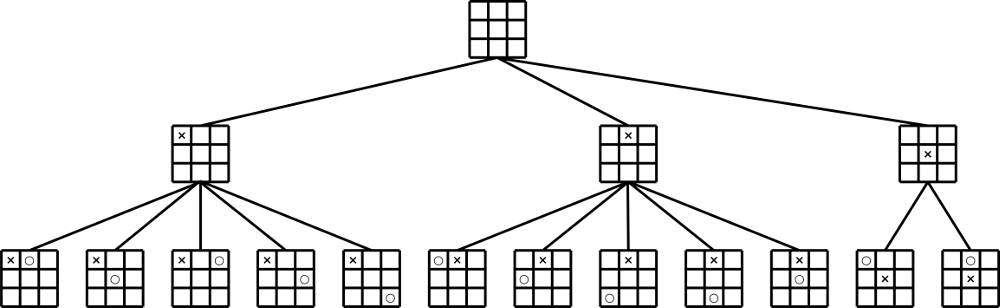
\includegraphics[width=\linewidth]{g59b.png}
				\end{center}
				\item[c.]对于深度为2的棋局,$X$和$O$均各只有一个,所以$X_2(s)=0$,$O_2(s)=0$,评估函数退化为:
				\begin{equation*}
					\text{Eval}(s)=X_1(s)-O_1(s)
				\end{equation*}
				分别计算各个棋局的评估函数值,计算结果如下:
				\begin{center}
					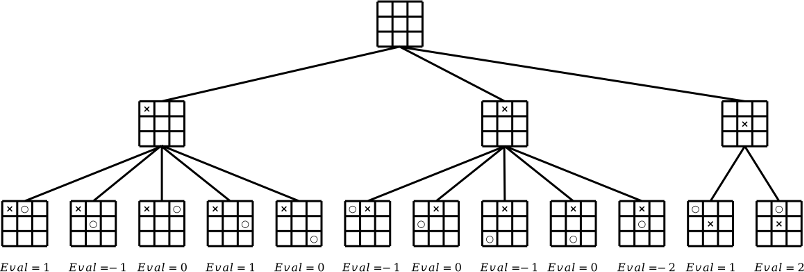
\includegraphics[width=\linewidth]{g59c.png}
				\end{center}
				\item[d.] 先计算深度为1的结点,再计算深度为0的结点:
				\begin{center}
                    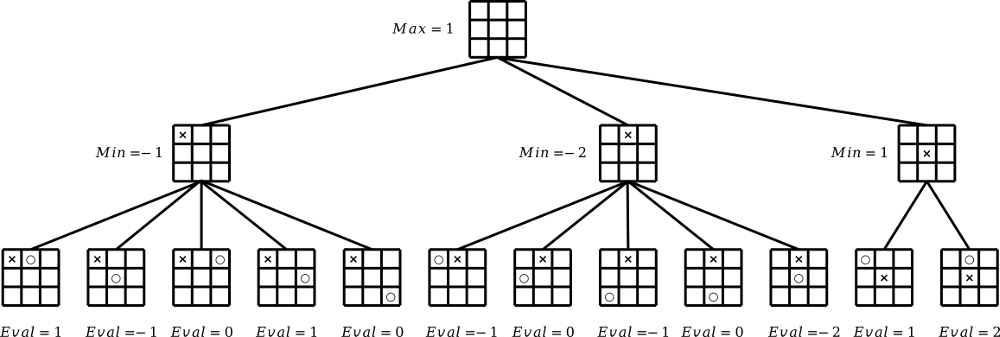
\includegraphics[width=\linewidth]{g59d.png}
                \end{center} 
                可以推断出,$X$第一步的最佳行棋是棋盘中间。
                \item[e.] 首先我们给所有的结点编上序号,分别为$A$到$P$。按照题目的假设,结点是按照对$\alpha$--$\beta$剪枝的最优顺序生成的,那么我们考察下图所示的最优的顺序之一:
                \begin{center}
                    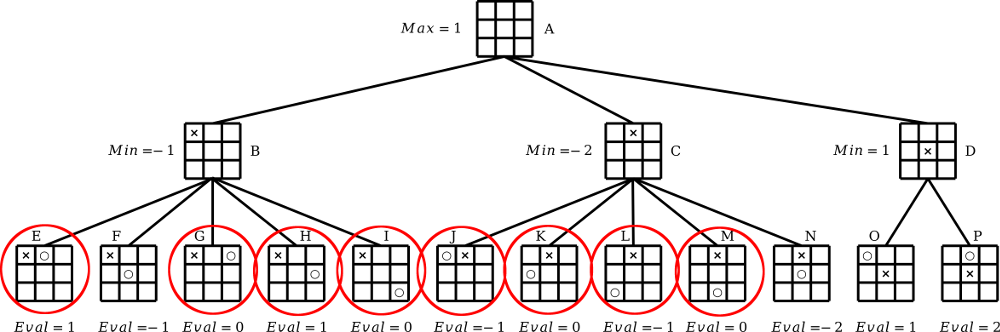
\includegraphics[width=\linewidth]{g59e.png}
                \end{center} 
                图中的顺序是这样的:先访问结点$O$,由于$O=1$,得知$D$的最大值是1。接下来看$P$,由于$P=2 > 1$,所以$D$结点的取值定为1。这时,$A$结点的最小值为1,我们希望在$B$和$C$中找到大于1的结点。假如我们先看$B$下的$F$结点,$F=-1$,所以$B$的取值最大才为$-1$,不可能大于1,所以$B$结点生成的其它结点($E,G,H,I$)可以全部剪掉。接下来再看$C$下的$N$结点,$N=-2$,因此$C$结点最大值为$-2$,同样没有超过1的可能,所以$C$下的其它结点($J,K,L,M$)也都要剪掉。所以最后$A$结点的取值就是1.
			\end{enumerate} 
        \item[5.8] 
        \begin{enumerate}
            \item[a.]按照题目要求的约定,画出的完整博弈树为:
                \begin{center}
                    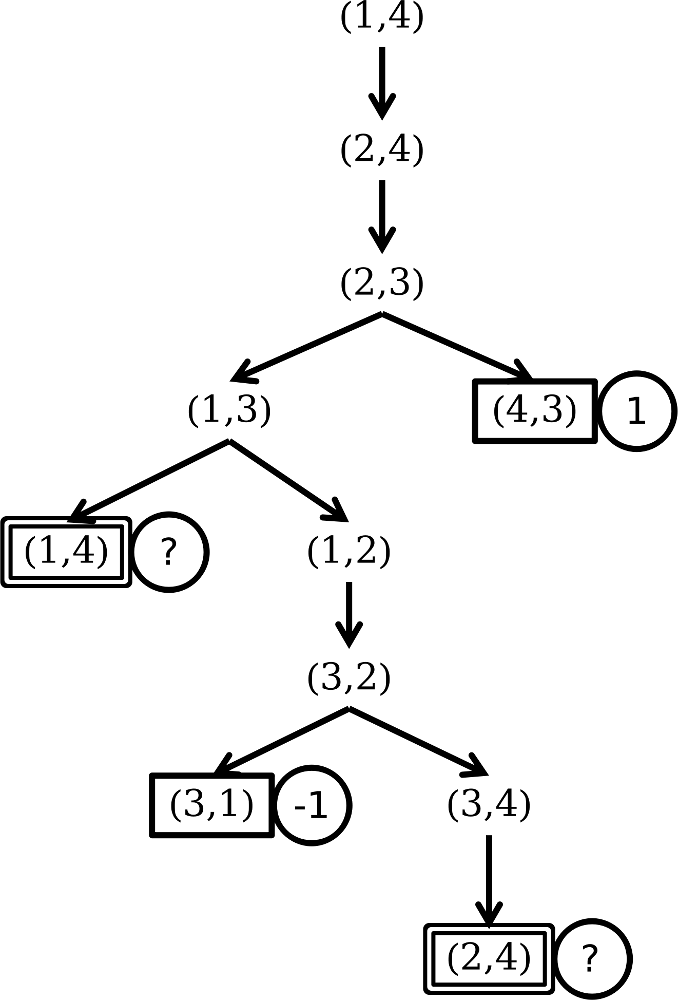
\includegraphics[height=10cm]{g58a.png}
                \end{center} 
            \item[b.]我们首先确定``?''以外的值。可以看出,这几个不确定的值对顶层结点的极小极大值完全没有影响。因为上层结点的结果是确定的,所以最后,我们可以把上层计算出来的极小极大值填写到底层的不确定的结点中:
            \begin{center}
                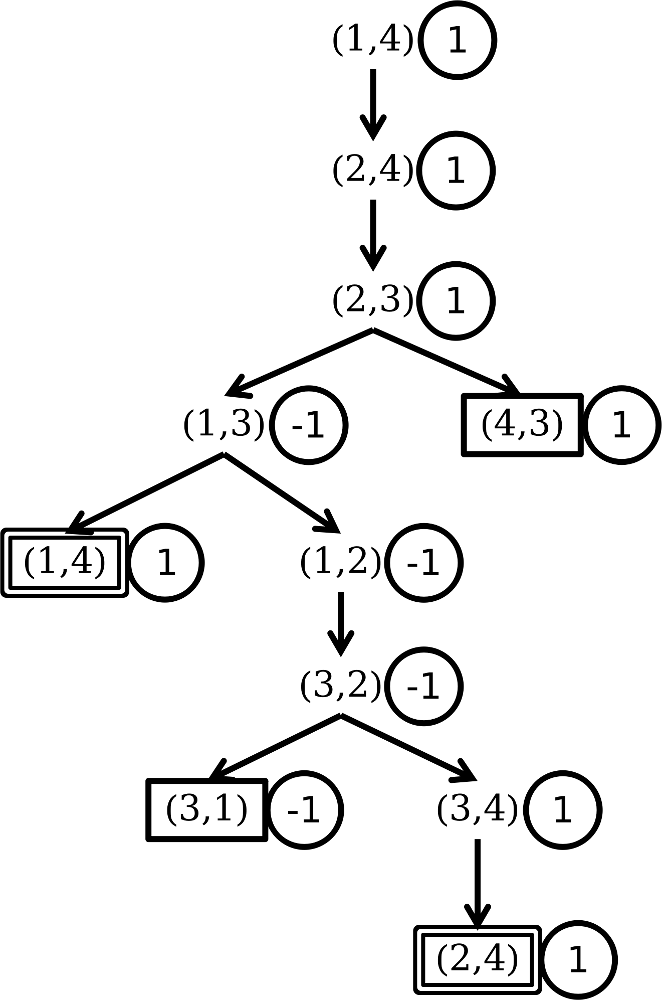
\includegraphics[height=10cm]{g58b.png}
            \end{center} 
            \pagebreak
            \item[c.]标准的极小极大算法是通过递归来穷举问题的,而这个问题存在循环的情况,没有办法通过穷举来达到尽头,所以标准的极小极大算法会失败。

            我的修正方案是:将已经遇到的状态存入称为“换位表”的哈希表中,当每次生成新的状态的时候,从换位表中查询该状态。如果该状态已经存在,并且还没有答案,则返回一个评估函数确定的结果(比如在这个问题里,可以是0)。

            对于所有包含循环的游戏,我修正后的算法不一定能得到最优决策。比如,在这个游戏里,几个``?''处恰好和1一起取最大值,和-1一起取最小值,无论``?''取什么值,都不影响最后的结果。但是对于其它一些包含循环的游戏,比如国际象棋,如果遇到循环,很难保证我的算法中的评估函数是最优的,也就没法保证最终的决策是最优的了。
            \item[d.] 首先对于$n=3$,双方的移动是唯一的,$A$向右走,$B$越过$A$到达最左边,$A$输。对于$n=4$,前面也讨论过了。下面只讨论$n\geq 5$的情况。

            $A$和$B$希望抢先到达对方游戏开始时所在的格子,所以$A$向右移动,$B$向左移动。

            如果$n$为奇数:$A$到达正中间时,$B$越过了$A$。如果$A$继续向右移动,则$B$将领先于$A$一步到达最左边的格子,所以$A$只能试图越过$B$向左,阻止$B$。如果$n=4k+1$,$A$最终会正好到达最左边的格子。此时接下来的移动几乎是唯一的:$B$向右移动一步,$A$只能向右移动一步,$B$越过$A$到达最左边的格子,$A$输了。
            \begin{center}
                \begin{tabular}{|c|c|c|c}
                    \hline
                    & $B$ & $A$ & $\cdots$ \\ \hline
                    $A$ & $B$ & & $\cdots$ \\ \hline
                    $A$ & & $B$ & $\cdots$ \\ \hline
                    & $A$ & $B$ & $\cdots$ \\ \hline
                    $B$ & $A$ & & $\cdots$ \\ \hline
                \end{tabular}
            \end{center}
            如果$n=4k+3$,则$B$最终正好到达最左边的格子,$A$也输了。
            \begin{center}
                \begin{tabular}{|c|c|c|c}
                    \hline
                    & $A$ & $B$ & $\cdots$ \\ \hline
                    $B$ & $A$ & & $\cdots$ \\ \hline
                \end{tabular}
            \end{center}
            如果$n$为偶数:情况和奇数时是对称的,如果$B$不管$A$,$A$会先到;如果$B$越过$A$向右,同样分为$A$恰好直接到达以及$B$到达最右边的格子两种情况,对于前一种,$B$直接输掉,对于后一种,$A$向左移动一步,$B$只能向左移动,$A$再越过$B$,到达最右边的空格,同样是$B$输掉。
        \end{enumerate} 
        \item[5.13]
        \begin{enumerate}
            \item[a.] 假设$n_1,n_2,...,n_{j-1}$分别有$b_2+1,b_3+1,...,b_j+1$个后代结点,有
            \begin{align*}
                n_1&=\min(n_2,n_{2\ 1},...,n_{2\ b_2}) \\
                n_2&=\max(n_3,n_{3\ 1},...,n_{3\ b_3}) \\
                n_3&=\min(n_4,n_{4\ 1},...,n_{4\ b_4}) \\
                \cdots & \cdots \\
                n_{j-1}&=\min(n_j,n_{j\ 1},...,n_{j\ b_j})
            \end{align*}
            把下面的式子代入到上面的式子中,得到
            \begin{align*}
                n_1&=\min(n_2,n_{2\ 1},...,n_{2\ b_2}) \\
                   &=\min(\max(n_3,n_{3\ 1},...,n_{3\ b_3}),n_{2\ 1},...,n_{2\ b_2}) \\
                   &=\min(\max(\min(n_4,n_{4\ 1},...,n_{4\ b_4}),n_{3\ 1},...,n_{3\ b_3}),n_{2\ 1},...,n_{2\ b_2}) \\
                   &=\min(\max(\cdots\min(n_j,n_{j\ 1},...,n_{j\ b_j})\cdots,n_{3\ 1},...,n_{3\ b_3}),n_{2\ 1},...,n_{2\ b_2})
            \end{align*}
            \item[b.]从$n_1$开始:
            \begin{align*}
                n_1&=\max(l_2,n_2,r_2) \\
                n_2&=\min(l_3,n_3,r_3) \\
                n_3&=\max(l_4,n_4,r_4) \\
                \cdots&\cdots \\
                n_{j-1}&=\min(l_j,n_j,r_j)
            \end{align*} 
            把下面的式子代入上面的式子:
            \begin{align*}
                n_1&=\max(l_2,n_2,r_2)\\
                   &=\max(l_2,\min(l_3,n_3,r_3),r_2)\\
                   &=\max(l_2,\min(l_3,\max(l_4,n_4,r_4),r_3),r_2)\\
                   \cdots&\cdots \\
                   &=\max(l_2,\min(l_3,\max(l_4,\cdots\min(l_j,n_j,r_j)\cdots,r_4),r_3),r_2)
            \end{align*}
            \item[c.]如果$n_j$要对$n_1$产生影响,那么需要$n_j<l_j$,从而$\min(l_j,n_j,r_j)=n_j$,还需要$n_j>l_{j-1}$,从而$\max(l_{j-1,n_j,r_{j-1}})=n_j$,等等,一直到$n_2$,把这些约束全部写出来:
            \begin{equation*}
                \begin{cases}
                    n_j > l_2 \\
                    n_j < l_3 \\
                    \cdots\cdots \\
                    n_j > l_{j-1} \\
                    n_j < l_j
                \end{cases}
            \end{equation*} 
            \item[d.]如果$n_j$是MIN结点,则上面的过程依次进行改变。第一步:
            \begin{align*}
                n_1&=\min(n_2,n_{2\ 1},...,n_{2\ b_2}) \\
                   &=\min(\max(n_3,n_{3\ 1},...,n_{3\ b_3}),n_{2\ 1},...,n_{2\ b_2}) \\
                   &=\min(\max(\min(n_4,n_{4\ 1},...,n_{4\ b_4}),n_{3\ 1},...,n_{3\ b_3}),n_{2\ 1},...,n_{2\ b_2}) \\
                   &=\min(\max(\cdots\max(n_j,n_{j\ 1},...,n_{j\ b_j})\cdots,n_{3\ 1},...,n_{3\ b_3}),n_{2\ 1},...,n_{2\ b_2})
            \end{align*} 
            第二步:
            \begin{align*}
                n_1&=\max(l_2,n_2,r_2)\\
                   &=\max(l_2,\min(l_3,n_3,r_3),r_2)\\
                   &=\max(l_2,\min(l_3,\max(l_4,n_4,r_4),r_3),r_2)\\
                   \cdots&\cdots \\
                   &=\max(l_2,\min(l_3,\max(l_4,\cdots\max(l_j,n_j,r_j)\cdots,r_4),r_3),r_2)
            \end{align*}
            最后一步,$l_i$的约束:
            \begin{equation*}
                \begin{cases}
                    n_j > l_2 \\
                    n_j < l_3 \\
                    \cdots\cdots \\
                    n_j < l_{j-1} \\
                    n_j > l_j
                \end{cases}
            \end{equation*} 
        \end{enumerate}
	\end{itemize}
\end{document}